\documentclass[defaultstyle,10pt,master,Helvetica]{thesis}
%% Enable latin characters
\usepackage[utf8]{inputenc}

%% Better equations
\usepackage{amsmath, amsthm, amssymb, amsfonts}

%% Advanced tables
\usepackage{multirow}
\usepackage{colortbl}

%% Better figures
\usepackage{graphics}
\usepackage{epsfig}
\usepackage[hang,small,bf]{subfigure}

%% The two packages are not compatible, and you should use one of the two. Notice however that the
\usepackage[square,numbers,sort&compress]{natbib}

%% Acronyms
\usepackage[printonlyused]{acronym}

%% Set links for references and citations in document
\usepackage{hyperref}
\hypersetup{ a4paper=true,
             colorlinks=false,
             citecolor=red,
             breaklinks=true,
             bookmarks=true,
             bookmarksnumbered=true,
             bookmarksopen=true,
             pdftitle={DOCUMENT TITLE},                 % EDIT THIS LINE
             pdfauthor={THE AUTHOR},                    % EDIT THIS LINE
             pdfsubject={THE SUBJECT},                  % EDIT THIS LINE
             pdfcreator={THE PDF CREATOR - THE AUTHOR}, % EDIT THIS LINE
             pdfkeywords={}                             % EDIT THIS LINE
}

%% Set paragraph counter to alphanumeric mode
\renewcommand{\theparagraph}{\Alph{paragraph}~--}

%% Page formatting, edit if necessary
\hoffset 0in
\voffset 0in
\oddsidemargin 0.71cm
\evensidemargin 0.04cm
\marginparsep 0in
\topmargin -0.25cm
\textwidth 15cm
\textheight 23.5cm

\usepackage{fancyhdr}
\pagestyle{fancy}
\renewcommand{\chaptermark}[1]{\markboth{\thechapter.\ #1}{}}
\renewcommand{\sectionmark}[1]{\markright{\thesection\ #1}}
\fancyhf{} \fancyhead[LE]{\bfseries\nouppercase{\leftmark}}
\fancyhead[RO]{\bfseries\nouppercase{\rightmark}}
\fancyfoot[LE,RO]{\bfseries\thepage}
\renewcommand{\headrulewidth}{0.5pt}
\renewcommand{\footrulewidth}{0.5pt}
\addtolength{\headheight}{2pt} % make space for the rule
\fancypagestyle{plain}{%
   \fancyhead{} % get rid of headers
   \renewcommand{\headrulewidth}{0pt} % and the line
   \renewcommand{\footrulewidth}{0pt}
}
\fancypagestyle{blank}{%
   \fancyhf{} % get rid of headers and footers
   \renewcommand{\headrulewidth}{0pt} % and the line
   \renewcommand{\footrulewidth}{0pt}
}
\fancypagestyle{abstract}{%
   \fancyhead{}
   \renewcommand{\headrulewidth}{0pt}
   \renewcommand{\footrulewidth}{0.5pt}
}
\fancypagestyle{document}{%
	\fancyhf{} \fancyhead[LE]{\bfseries\nouppercase{\leftmark}}
	\fancyhead[RO]{\bfseries\nouppercase{\rightmark}}
	\fancyfoot[LE,RO]{\bfseries\thepage}
	\renewcommand{\headrulewidth}{0.5pt}
	\renewcommand{\footrulewidth}{0.5pt}
	\addtolength{\headheight}{2pt} % make space for the rule
}
\setcounter{secnumdepth} {5}
\setcounter{tocdepth} {5}
\renewcommand{\thesubsubsection}{\thesubsection.\Alph{subsubsection}}

\renewcommand{\subfigtopskip}{0.3 cm}
\renewcommand{\subfigbottomskip}{0.2 cm}
\renewcommand{\subfigcapskip}{0.3 cm}
\renewcommand{\subfigcapmargin}{0.2 cm}


\begin{document}
\pdfbookmark[0]{Titlepage}{Title}
% IST requires the titlepage to be written in portuguese
% IST requires the logo to measure 2cm
\univlogo{3cm}{2cm}{images/IST_C_CMYK_POS.eps}

% OPTIONAL: the thesis logo image
\thesislogo{2.5cm}{6cm}{images/thesis_logo.eps}

\title{A IST stylesheet example for writing dissertations}

\author{Pedro Tom\'as}
\degree{Engenharia Electrot\'ecnica e de Computadores}
% \otherdegree{Mestre}

\supervisor{Doutor full name of advisor}
% \othersupervisor{Doutor full name of co-advisor}

\date{Outubro de 2014}

% Only true if thesis was accepted by the jury
\finalthesis{false}

\presidentofjury{Doutor whatever full name 1}
\vogalone{Doutor whatever full name 2}
\vogaltwo{Doutor whatever full name 3}
% \vogalthree{Doutor whatever full name 4}
% \vogalfour{Doutor whatever full name 5}

\maketitle
\clearpage

% On double sided pages. Second page should be white.
% IST requires the cover to appear twice.
\thispagestyle{empty}
\cleardoublepage

\setcounter{page}{1} \pagenumbering{roman}

\baselineskip 18pt % line spacing: -12pt for single spacing
                   %               -18pt for 1 1/2 spacing
                   %               -24pt for double spacing
 
\pdfbookmark{Acknowledgments}{Acknowledgments}
\begin{acknowledgments}
Remember that your parents have paid for the last 20 something years of your studies and that your advisor had to read this document.
\end{acknowledgments}
 

\pdfbookmark{Abstract}{Abstract}

\begin{abstract}
 %TODO ADD: social data has very few text but a lot hidden signals 
 %          tweets in particullar have even few text, makes them harder to cathegorize
  Clustering is a widely used technique in data analysis. In this thesis, a generically \acrodef{ANN}[artificial neural network] algorithm used for clustering is modified in order to enhance the value of socially connected ententies.

To achieve this, we present RubySOM. A framework for easy construction of custom Self-Organizing Maps. With it, it is possible to dinammically change multiple parts of the algorithm, making it extremlly flexible solution to create, train and run custom implementations of the algorithm. 

With RubySOM, a relational aware version of the SOM algorithm was created in order to better identify topics on the social network twitter. 
\end{abstract}

\begin{keywords}
topic detection, twitter, self-organizing maps, classification, clustering
\end{keywords}
\clearpage
\thispagestyle{empty}
\cleardoublepage

\pdfbookmark{Resumo}{Resumo}
\begin{resumo}

\end{resumo}

\begin{palavraschave}
  detecção de tópicos, twitter, mapas auto organizados, classificação, agrupamento
\end{palavraschave}

\clearpage
\thispagestyle{empty}
\cleardoublepage

% Required for the fancy chapters
\dominitoc
\dominilof
\dominilot
 

%%%%%%%%%%%%%%%%%%%%%%%%%%%%%%%%%%%%%%%%%%%%%%%%%%%%%%%%%%%%%%%%%%%%%%
% List of contents
%\renewcommand{\baselinestretch}{1}
\pdfbookmark[0]{Index}{index}
\pdfbookmark[1]{Contents}{toc}
\tableofcontents
% \contentsline{chapter}{References}{\pageref{bib}}
\cleardoublepage
%\renewcommand{\baselinestretch}{1.5}

%%%%%%%%%%%%%%%%%%%%%%%%%%%%%%%%%%%%%%%%%%%%%%%%%%%%%%%%%%%%%%%%%%%%%%
% List of figures
\pdfbookmark[1]{List of Figures}{lof}
\listoffigures
\cleardoublepage

%%%%%%%%%%%%%%%%%%%%%%%%%%%%%%%%%%%%%%%%%%%%%%%%%%%%%%%%%%%%%%%%%%%%%%
% List of tables
\pdfbookmark[1]{List of Tables}{lot}
\listoftables
\cleardoublepage

% %%%%%%%%%%%%%%%%%%%%%%%%%%%%%%%%%%%%%%%%%%%%%%%%%%%%%%%%%%%%%%%%%%%%%%
% % List of algorithms
% Requires packages algorithmic, algorithm
% \pdfbookmark[1]{List of Algorithms}{loa}
% \listofalgorithms
% \cleardoublepage

% %%%%%%%%%%%%%%%%%%%%%%%%%%%%%%%%%%%%%%%%%%%%%%%%%%%%%%%%%%%%%%%%%%%%%%
% % List of acronyms
\makeglossaries
\pdfbookmark[1]{List of Acronyms}{loac}
\markboth{List of Acronyms}{List of Acronyms}
\chapter*{List of Acronyms}
% This is the ACRONYMS Definition
\begin{acronym}[TDMA]
	\acro{SOM}{Self-Organizing Maps}
	\acro{NLP}{Natural Language Processing}
	\acro{U-Matrix}{Unified Distance Matrix}
	\acro{TF-IDF}{Term Frequency–Inverse Document Frequency}
	\acro{BMU}{Best Matching Unit}
	\acro{LDA}{Latent Dirichlet Allocation}
	\acro{TDT}{Topic Detection and Tracking}
	\acro{VSM}{Vector Space Model}
	\acro{IR}{Information Retrieval}
	\acro{ML}{Machine Learning}
	\acro{ANN}{Artificial Neural Network}
	\acro{MDS}{Multi Dimensional Scalling}
	\acro{PCA}{Principle Component Analysis}
	\acro{URL}{Uniform Resource Locator}
	\acro{JSON}{JavaScript Object Notation}
	\acro{CSV}{Comma Separated Values}
	\acrodefplural{SOM}[SOMs]{Self Organizing Maps}
	\acrodefplural{ANN}[ANNs]{Artificial Neural Networks}
\end{acronym}

\cleardoublepage

% Change pagination from Roman to Arabic.
\setcounter{page}{1} \pagenumbering{arabic}
\baselineskip 18pt
 

\fancychapter{Introduction}
 With the evolution of social network websites like Facebook and Twitter, the amount of pertinent content about a specif issue is increasing dramatically, which calls for new ways to make sense and catalog this data.
The usage of social networks for branding quality and on-line marketing is specially compelling since 19\% of all tweets ~\cite{Jansen2009} and 32\% ~\cite{Melville2009} of blog posts are about brands or products.
On the other hand, finding topic sensitive information on social networks is extremely complicate due to the fact that documents have very little content, slang vocabulary and orthographically mistakes or abbreviations.

~\citet{Asur2010} successfully predicted box-office revenues by monitoring the rate of creation of new topics based on debuting movies. ~\citet{Asur2010} was able to outperformed some market-based predictors.

Academic and enterprise world is now starting to look at Machine Learning for new ways to achieve revenue and visualize data representing the way the world works. 
As a consequence, the Machine Learning course at Standford is the one with more students enrolling this year \footnote{http://www.forbes.com/sites/anthonykosner/2013/12/29/why-is-machine-learning-cs-229-the-most-popular-course-at-stanford/} with more than 760 students enrolled.

 ~\cite{Le2011} was able to achieved 81.7 percent accuracy in detecting human faces, 76.7 percent accuracy when identifying human body parts and 74.8 percent accuracy when identifying cats. He used a 9-layered locally connected sparse auto-encoder with pooling and local contrast normalization on a large dataset of images (the model has 1 billion connections, the dataset has 10 million 200x200 pixel images downloaded from the Internet) trained using model parallelism and asynchronous SGD on a cluster with 1,000 machines (16,000 cores) during three days. Even though the amount of computing power used in this project was of several order of magnitude, it is remarkable how an unsupervised algorithm could achieve such results.

Even though a lot of solutions have arisen in order to automate real time searches, topic categorization and many other data intensive tasks, Twitter still uses humans in order to deliver ads to trending queries states Edwin Chen's Data Scientist Responsible for ads quality at Twitter. On his blog post \footnote{http://blog.echen.me/2013/01/08/improving-twitter-search-with-real-time-human-computation/} Edwin describes the process of Twitter to deliver real time adds to trending queries, the main problems that arise in the Twitter platform in order to identify rising topics are mainly:
\begin{itemize}
  \item The queries people perform have never before been seen, so it's impossible to know beforehand what they mean.
  \item Since the spikes in search queries are short-lived, there's only a short window of opportunity to learn what they mean.
\end{itemize}
This means that when an event happen, people immediately come to Twitter in order to know what is happening in a determined place in real time. Twitter solves this issue by monitoring which queries are currently popular in real time, using a Storm topology \footnote{http://storm-project.net/} and after the queries are identified, they are sent to a Thrift API \footnote{http://thrift.apache.org/} that dispatches the query to Amazon's Mechanical Turk \footnote{https://www.mturk.com/mturk/} service where real people will be asked a variety of questions about the query.

Social Media Analytics is another raising topic which draws from Social Network Analysis, Machine Learning, Data Mining, Information Retrieval (IR), and Natural Language Processing (NLP). As stated by Melville et al. in ~\cite{Melville2009} 32\% of the 200 million bloggers world wide blog about opinions on products and brands, 71\% of the 625 million active Internet users actually read blogs and more importantly that 78\% of respondents put their trust in the opinion of other consumers where only only 57\% of consumers trust advertising in traditional media and even worst only 34\% of consumers put their trust in such advertising. This kind of data drives companies to Social Media Analytics in a way to know what people are saying on the web about their companies and products. This new worry has brought to life a lot of new startups like Sumal\footnote{https://sumall.com/} or ThoughtBuzz\footnote{http://www.thoughtbuzz.net/} but also solutions from the old players like IBM \footnote{http://www-01.ibm.com/software/analytics/solutions/customer-analytics/social-media-analytics/} and SAS \footnote{http://www.sas.com/software/customer-intelligence/social-media-analytics.html}

Its also important to notice that in the last few years Data Science/Analysis has been a trending topic, mostly due to the fact that big dot-com companies have been making lots of money through exploiting user specific information in order to deliver ads and sell products. No wonder that if you look that in the top 10 ebooks sold by O'Reilly throughout 2013, four are about data science \footnote{http://shop.oreilly.com/category/deals/best\-of\-oreilly\-dotd.do?code=DEAL\&cmp=tw\-na\-books\-videos\-info\-authornote\_best\_of\_2013}.

In this project we will focus on using an unsupervised learning technique based on neural networks named Self-Organizing Maps ~\cite{Kohonen1990} in order to detect topics in Twitter posts, by using the Social Network users as base neurons for clustering. After the network is trained, it will be possible to categorize tweets in real time. This approach will be better described in subsection ~\ref{sub:objectives}.

This document is organized as follows. First will be dedicated to explain some basics concepts like Document CLustering and specifically Self-Organizing Maps in Section ~\ref{sec:basic_concepts}.  Further in, Section ~\ref{sec:related_work} will be dedicated to the state of the art solutions related not only to topic detection but also to twitter data analysis and Self-Organizing Maps.In Section ~\ref{sec:architecture} Architecture of the purposed solution and  at Section ~\ref{sec:evaluation_metrics} it will be discussed how to evaluate results achieved. Finally we will this report by referencing some possible future work and with a brief conclusion at Section ~\ref{sec:coclusions_future_work}.
 
%TODO Check if Im Answering these questions
\begin{enumerate}
 \item what is the background of your work?
 \item how do your work fit in todays knowledge? Have you done something that does not exist in the market? What are the differences? What is missing in nowadays products and solutions?
 \item is your thesis made as part of a larger project? If so, describe it.
 \item is your thesis usefull for some work environment? If so, describe it.
\end{enumerate}

\section{Motivation}

%TODO I dont have motivation
Given the general description provided previously, what is the motivation of your work. Explain why the product or solution developed in the course of your thesis is important.

\section{Objectives}

%TODO Change text to what Ive actually done
The objective of this project is clear: finding topics on Tweets by analyzing their textual specific characteristics, like number of characters in a tweet, hashtags, is a retweeted \footnote{retweet is when a user shares a tweet that is not his}, etc., and contextualize the social network involving the person that did the tweet by retrieving user specific profile information.

After building the dataset, it will be needed to train the Self-Organizing map neural network in order to be able to have the network ready for clustering classification of each future tweet that will be added to it. After the SOM training it will be necessary to categorize the clusters in order to know which topic they belong to. When this step ha ended it will be possibly to get new tweets categorized on the moment they enter the network without further delay.

Finally it will be presented a website where a user will be able to login with his twitter account and see all of his tweets being categorization in the moment they are clustered. After all the user tweets are clustered there will a graphical presentation of the user twitter usage where it will be possible to see multiple statistical information such as the the topics a user is more interested in and his own twitter Self-Organizing map network of topics with his friends, the wire-frames of the website can be seen in the attachments Section ~\ref{sec:attachments} in Figure ~\ref{fig:wireframes}.
 

\section{Main contributions}
%TODO Explain all the open source lybraries that Ive published
Do not forget this one. Notice that the objectives is what you have proposed to do. Main contributions are the innovations of your work, or, in other cases, what your work is really good at. If you submitted/published an article in a peer-reviewed conference or journal, do not forget to state here.

\section{Dissertation outline}
%TODO Write the outline
Explain how did you organized your thesis.

\cleardoublepage 

\fancychapter{State of the art}
The second chapter can be the state of the art for the work you are preenting. Sometimes it appears under the previous chapter -- Introduction. Though I typically prefer to put it in a separate chapter.

In most cases this chapter addresses some important technology or knowledge. Name this chapter according to the topic.

The introduction should be written assuming that the reader has little or no knowledge of your specific problem. Try to write this chapter in a clear manner that makes it easier for the reader to understand the remaining of your thesis. Append information to this chapter as needed when writting other chapters.

Do not forget to add references to your document. In general, if you are stating something which is not obvious nor it is of common knowledge amongst the scientific or engineering community, you should place a reference. To ease the process of referencing I include a couple of references to my own papers herein. Here are some examples: \cite{tomas2010bda}, \citep{tomas2010aqa}, \citet{ramalho2010eic}, \mbox{\cite[(2.2)]{tomas2009nct}}.

To help you make references, you can try the commands or consult the manual. The following link can also be a good help:
\mbox{\underline{http://merkel.zoneo.net/Latex/natbib.php}}.

As a side note, remember that you should not include links in your dissertation as I just made. Instead you should put a reference as follows: \cite{mylink}. Remember that in this case, the reference date is the date you have last consulted the page.

\section{Summary}

It is typical a good ideia to have an ending section summarizing the chapter.

% Ensure that the next chapter starts in a odd page
\cleardoublepage 

\fancychapter{The work}

{\color{red}\bfseries IMPORTANT NOTICE: This chapter should not be called ``The Work'' in the final version of your dissertation. This comment was inserted after some of my faculty collegues noticed that some naive souls call the chapter ``The Work''. This is by no means appropriate. This and all chapter names should be named accordingly to your thesis.}

The third chapter is typically the work you have performed in your thesis. Obviously you should focus on your contributions, but do not forget to write it so that others can understand. Never assume the reader knows the subject (unless it is really obvious). Your work is typically done in a very specific area which others may not know as much. So try to make it as clear as possible; and a self-explaining figure is always a big help.

\begin{figure}[t]
\centering
\subfigure[caption for subfigure a]{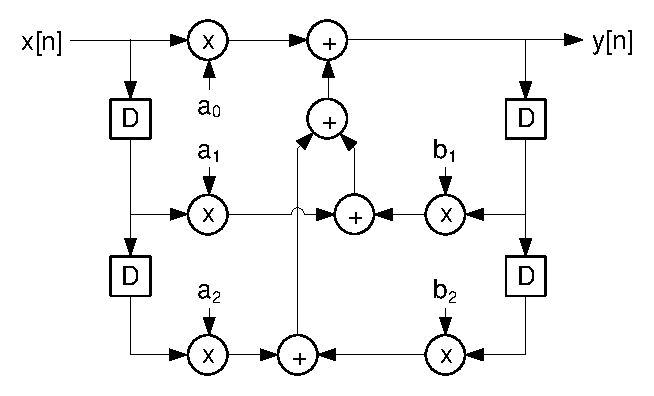
\includegraphics[scale=0.65]{images/img1.eps}\label{chp3:img1}}
\hspace*{0.5cm}
\subfigure[caption for subfigure b]{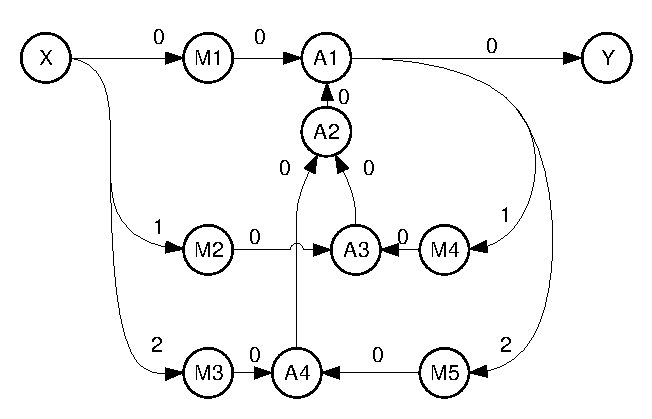
\includegraphics[scale=0.65]{images/img2.eps}\label{chp3:img2}}\\
\caption{A figure example.}
\label{fig:rmain figure}
\end{figure}

See the source code to see how to reference each of the subfigures \ref{chp3:img1} or \ref{chp3:img2}, or the main figure \ref{fig:rmain figure}.

There are several ways to define formulas (see the \textit{Short Math Guide for LaTeX} included in the package). The typical method is to use (see source code): 
\begin{equation}
a= b + c
\end{equation}
or
\begin{align}
c &= d \cdot e \nonumber\\
d &= \mathbf{X}^{\mathsf{T}} \mathbf{Y}+ \gamma e^{2\pi}
\label{chp3:eq1} 
\end{align}
or
\begin{subequations}
\begin{align}
c &= d \cdot e \label{chp3:eq2:a} \\
d &= \mathbf{X}^{\mathsf{T}} \mathbf{Y} + \gamma e^{2\pi}
\label{chp3:eq2:b} 
\end{align}
\label{chp3:eq2} 
\end{subequations}
where $\mathbf{X}$ and $\mathbf{Y}$ are column vectors (you should always present the meaning of each parameter). The \textbf{AMS} packages allow to use the command \verb"\eqref" to cite equations such as \eqref{chp3:eq1},  \eqref{chp3:eq2:a},\eqref{chp3:eq2:b} or \eqref{chp3:eq2} (see source code).

\section{Summary}

It is typical a good ideia to have an ending section summarizing the chapter.

% Ensure that the next chapter starts in a odd page
\cleardoublepage
 

 \fancychapter{Implementation}
 %TODO how it was implemented
I have no idea what to write here\dots

\begin{figure}
\begin{boxedverbatim}
DefineGlobals
   clock   alias   clk
   reset   alias   rst
   max_latency     17
   feedback        0
   DefineInputs
      X   std_logic_vector(11 downto 0)
   EndInputs
   DefineOutputs
      Y   std_logic_vector(11 downto 0)
   EndOutputs
EndGlobals
\end{boxedverbatim}
\caption{An example code section.}
\label{chp4:img}
\end{figure}

Figure~\ref{chp4:img} shows an example of a \verb"\boxedverbatim" section. It allows to put blocks of code within a frame. I think makes a prettier printing.

\section{Summary}

An ending section summarizing the chapter, is typically a good idea.

% Ensure that the next chapter starts in a odd page
\cleardoublepage


\fancychapter{Results}

\section{Evaluation Metrics} 
\label{sec:evaluation_metrics}
Evaluation of the topic detection on Tweets will be made in two distinct ways. The first way will focus on  binary classification using the precision and recall metrics, and will be described in Subsection~\ref{sub:testing_for_precision_and_recall}. The second way will focus on statistically testing the SOM learning process and the computed trained network. This testing process will be described in Subsection~\ref{sub:cluster_quality_testing}. 

\subsection{Testing for Precision and Recall} 
\label{sub:testing_for_precision_and_recall}
Precision and Recall are both ways to measure the rate of right guesses made by the trained SOM network, and are defined in the following way:
\begin{itemize}
  \item \textbf{Precision:} Fraction of retrieved instances that where relevant 
    \begin{equation}
      precision = \frac{|{relevant\;documents}\cap{retrieved\;documents}|}{{retrieved\;documents}}
    \end{equation} 
  \item \textbf{Recall:} Fraction of relevant instances that where retrieved
   \begin{equation}
      recall = \frac{|{relevant\;documents}\cap{retrieved\;documents}|}{{relevant\;documents}} 
    \end{equation} 
\end{itemize}

In order to calculate Precision and Recall we need to have the \emph{relevant documents} and the \emph{retrieved documents}. The \emph{relevant documents} are rather hard to determine because they need to be categorized by humans, which is a tedious task. Until the writing of this document, only one free dataset categorized by hand was found\footnote{http://www.sananalytics.com/lab/twitter-sentiment/}, but it is categorized in sentiments and not by topics which makes it irrelevant for this project. If no dataset is found until the end of this project, a small dataset might be created in order to measure precision and recall.

\subsection{Statistically Testing the SOM} 
\label{sub:cluster_quality_testing}
SOM training is always subject to some variability due to multiple causes, like the sensitivity of initial conditions, convergence to local minima and sampling variability, as stated by ~\citet{Bodt}. This subsection will present statistical tools to measure the quality of the SOM, by measuring its quantization error and topology preservation.

\subsubsection{Quantization Error} 
\label{ssub:quantization_error}
The SOM Quantization Error is the mean of all Euclidean distances between the observed data points and their corresponding winning neuron. This value might vary depending on the initialization neurons or the order of the input data fed into the SOM while the training is occurring. When applied to an individual input data, represents how well a neuron is representing input data. Since the SOM Quantization Error represents the mean of all quantization errors from all the input data, generally, the lower the error is the best the SOM was trained.
\\
No general formula exists to minimize quantization error\cite{Bodt} . What is generally done is just to change the number and values of the starting neurons and the order of the input data in order to train multiple SOMs. In the end the SOM with the lowest quantization error is chosen.
In this project since multiple approaches to the SOM algorithm and data representation will be tested, as described in Section~\ref{ssub:default_som_approach_},and the ones having the lower quantization error will be selected for the prototype.

\subsubsection{Topology Preservation} 
\label{ssub:topology_preservation}
The Self-Organizing Map performs a mapping from the n-dimensional input space into the two dimensional output space and where resides one the most fascinating characteristics, which is that the output map tries to preserve the topology from the input space. This grants the SOM algorithm a way to visualize high-dimensional data that other neural networks or clustering algorithms don't have. Even though this is true, sometimes during training it is not possible to preserve the topology of the network.
Thus topology preservation can be measured through the Topographic error~~\citet{Kiviluoto1996} which is the proportion of all data vectors for which first and second BMUs \footnote{unit that is closest to the winning neuron. BMU Best fitting unit } are not adjacent units.
In this project the Topographic Error will be calculated for all SOM implementations and VSM usages in order to understand if the representation of the SOM output space is well defined.


\section{The results}
Usualy a future work section is presented here.
Finish your thesis with the experimental results.

\section{Summary}

An ending section summarizing the chapter is typical a good idead.

% Ensure that the next chapter starts in a odd page
\cleardoublepage
 

\fancychapter{Conclusions}
Draw your conclusions here and sell your work. Trasmit to the juri how hard it was to develop the presented work.


\section{Future work}
A future work section is usually here.

% Ensure that the next chapter starts in a odd page
\cleardoublepage
 

% Add Bibliography to the PDF table of contents (not the document table of contents)
\pdfbookmark[0]{Bibliography}{bib}
% The bibliography style sheet
% \bibliographystyle{IEEEtran}
\bibliographystyle{apalike}
% \bibliographystyle{unsorted}
% The BiBTeX file
\bibliography{bibliographies/biblio.bib}
\cleardoublepage   

\appendix
% %%%%%%%%%%%%%%%%%%%%%%%%%%%%%%%%%%%%%%%%%%%%%%%%%%%%%%%%%%%%%%%%%%%%%%
% First appendix
% %%%%%%%%%%%%%%%%%%%%%%%%%%%%%%%%%%%%%%%%%%%%%%%%%%%%%%%%%%%%%%%%%%%%%%
\fancychapter{Appendix A}
\label{ch:rsom_training}
\begin{figure}[htpb]
  \centering
  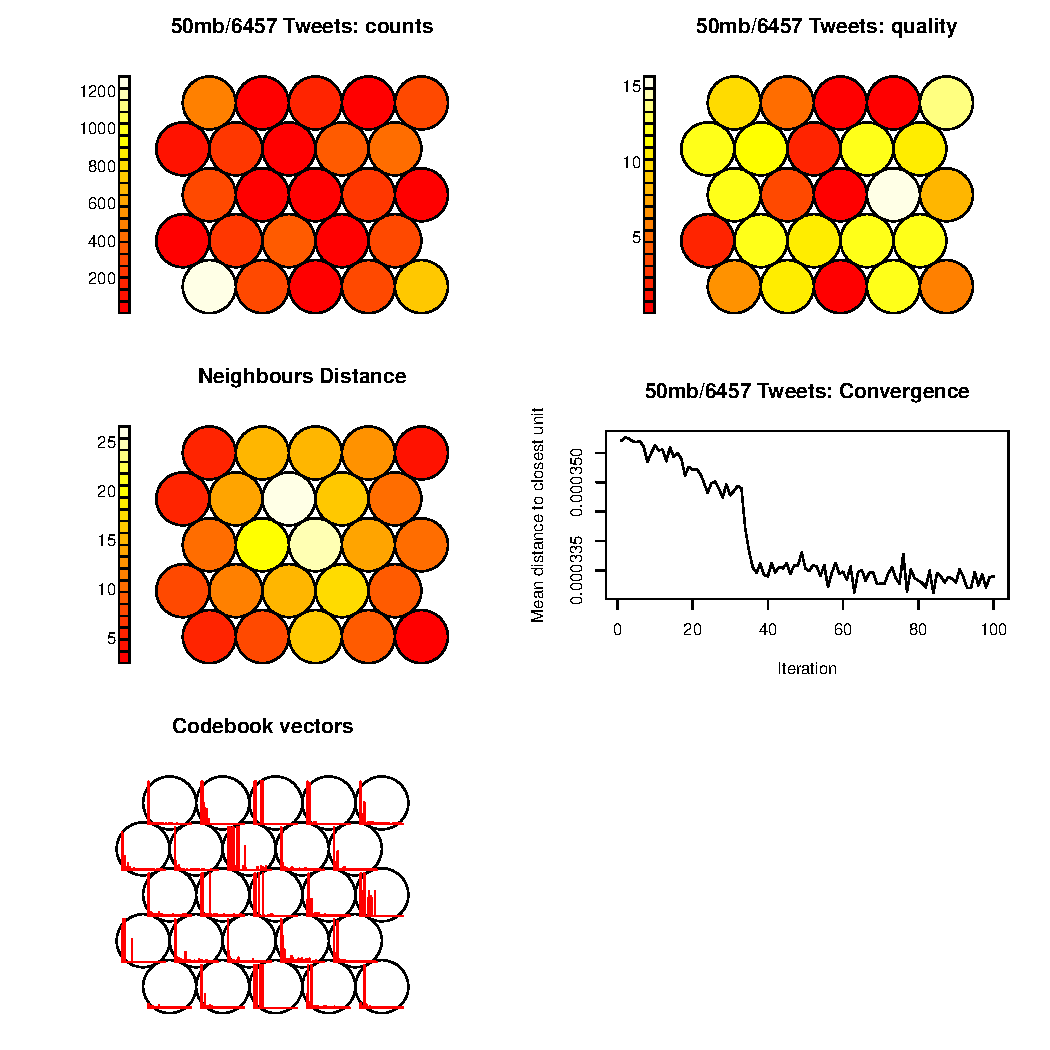
\includegraphics[width=0.8\linewidth]{./images/50mb_6457tweets_dataset.pdf}
  \caption{Training data for 6457 tweets. The counts map, shows us how many tweets are mapped to each cluster. Quality shows the mean distance of objects mapped to a unit to the codebook vector, the smaller the distance the better the representation. The neighborhood disance show the U-Matrix and finally the tweets convergence shows the distance from each node's wheights to the samples represented by that node }
  \label{fig:somr_images}
\end{figure}

\cleardoublepage

% %%%%%%%%%%%%%%%%%%%%%%%%%%%%%%%%%%%%%%%%%%%%%%%%%%%%%%%%%%%%%%%%%%%%%%
% Second appendix
% %%%%%%%%%%%%%%%%%%%%%%%%%%%%%%%%%%%%%%%%%%%%%%%%%%%%%%%%%%%%%%%%%%%%%%
%\fancychapter{Appendix A}
%\cleardoublepage  

\end{document}
